\documentclass{article}
\usepackage{graphicx}
\graphicspath{ {./} }
\usepackage[rightcaption]{sidecap}
\usepackage{wrapfig}
\usepackage[utf8]{inputenc}
\usepackage[utf8]{inputenc}
\usepackage[spanish]{babel}
\title{}
\author{}
\date{}
\pdfinfo{%
  /Title    (Intérprete de BOT - Etapa 1)
  /Author   (Meggie Sánchez, Jorge Marcano)
}
\begin{document}

\vspace{1.5cm}
 
\title{ 
\includegraphics[scale=0.3]{usb}  \\ Intérprete de BOT \\ Etapa 1 \\ Analizador Lexicográfico }

\author{Meggie Sánchez 11-10939, Jorge Marcano 11-10566} 

\date{20/09/2015}

\maketitle

\newpage

\section{Introducción}
\hspace{0.5cm} 	En el presente proyecto, se nos ha pedido crear un intérprete para el lenguaje llamado “BOT”. El desarrollo para el intérprete se dará en 4 etapas: (I) Análisis lexicográfico, (II) Análisis sintáctico y construcción del árbol sintáctico abstracto, (III) Análisis de contexto e (IV) Intérprete final del lenguaje. \\

Para la primera etapa, la implementación del analizador lexicográfico para el lenguaje BOT, ha sido realizada en el lenguaje de programación Python (versión 3.4), con la herramienta ofrecida por este mismo llamada PLY. 

\section{Implementación}
\hspace{0.5cm} Para la implementación del analizador lexicográfico, se utilizó como base los ejemplos mostrados en la documentación de la herramienta PLY. \\

Para mayor encapsulamiento y versatilidad, se decidió crear una clase BotLexer, de manera que las instancias de esta clase, sirvan como lexers para el lenguaje. En ésta clase se encuentra una lista de palabras reservadas, en la cual hemos incluido todas las palabras reservadas para operaciones del lenguaje. También se encuentra una lista de tokens, los cuales serán identificados y separados por medio del uso de expresiones regulares que los representen, algunos de estos tokens son simples signos de puntuación, y otros, más complicados, requieren del uso de funciones específicas para su reconocimiento, como es el caso por ejemplo de los identificadores de variables, y por último, tambien se encuentra la variable t\_ignore que ignora todos los tokens especificados en el lenguaje BOT. \\

Adicionalmente, en la clase BotLexer se ha incluido la función tokenizar(), la cual al ser llamada, tokeniza la entrada que se le dio al lexer e introduce los tokens en la lista toks, y los errores en la lista errors. Se tomó la decisión de hacer esto para poder tener los tokens y errores en estructuras separadas, para de esta manera poder usarlos para lo que sean necesarios, en este caso, imprimirlos.

\newpage

\section{Revisión Teórico-Práctica}
\subsection{Pregunta 1}
\hspace{0.5cm} Las tres expresiones regulares que corresponden respectivamente al reconocimiento de la palabra clave create es E1 = create, de la palabra char es E2 = char y de identificadores es E3 = [a-zA-Z][a-zA-Z\_0-9]* . 

\subsection{Pregunta 2}
\hspace{0.5cm} 
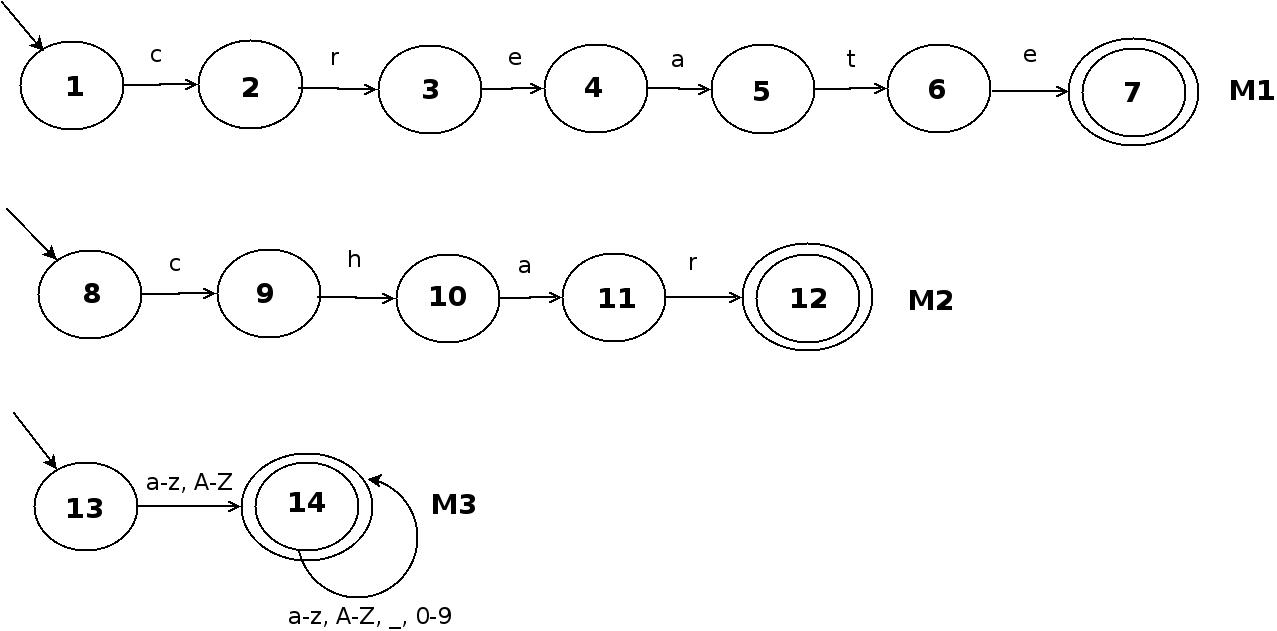
\includegraphics[scale=0.3]{preg2} 

\subsection{Pregunta 3}
\hspace{0.5cm}
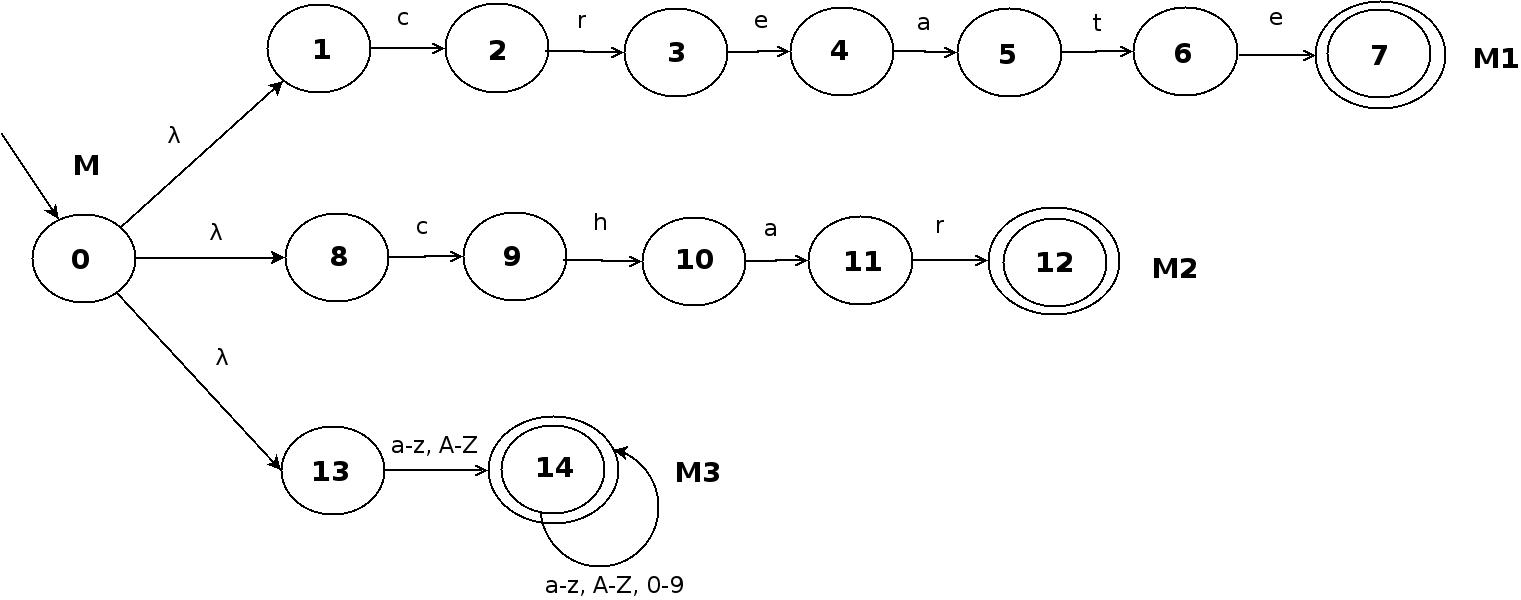
\includegraphics[scale=0.3]{preg3} 

\subsection{Pregunta 4}
\hspace{0.5cm} Para el autómata no-determinístico M, para el lenguaje L(M1) corresponde el estado final 7, para L(M2) corresponde el estado final 12, y por último, para L(M3) corresponde el estado final 14.

\subsection{Pregunta 5}
\hspace{0.5cm} Para nuestro autómata M, los conflictos son de L(M3) con L(M1) y L(M3) con L(M2). Las palabras que los generan son: para el primer caso, es create del lenguaje L(M1), y para el segundo caso, es char del lenguaje L(M2). Los estados finales involucrados son el 7, el 12 y el 14.

\subsection{Pregunta 6}
\hspace{0.5cm}
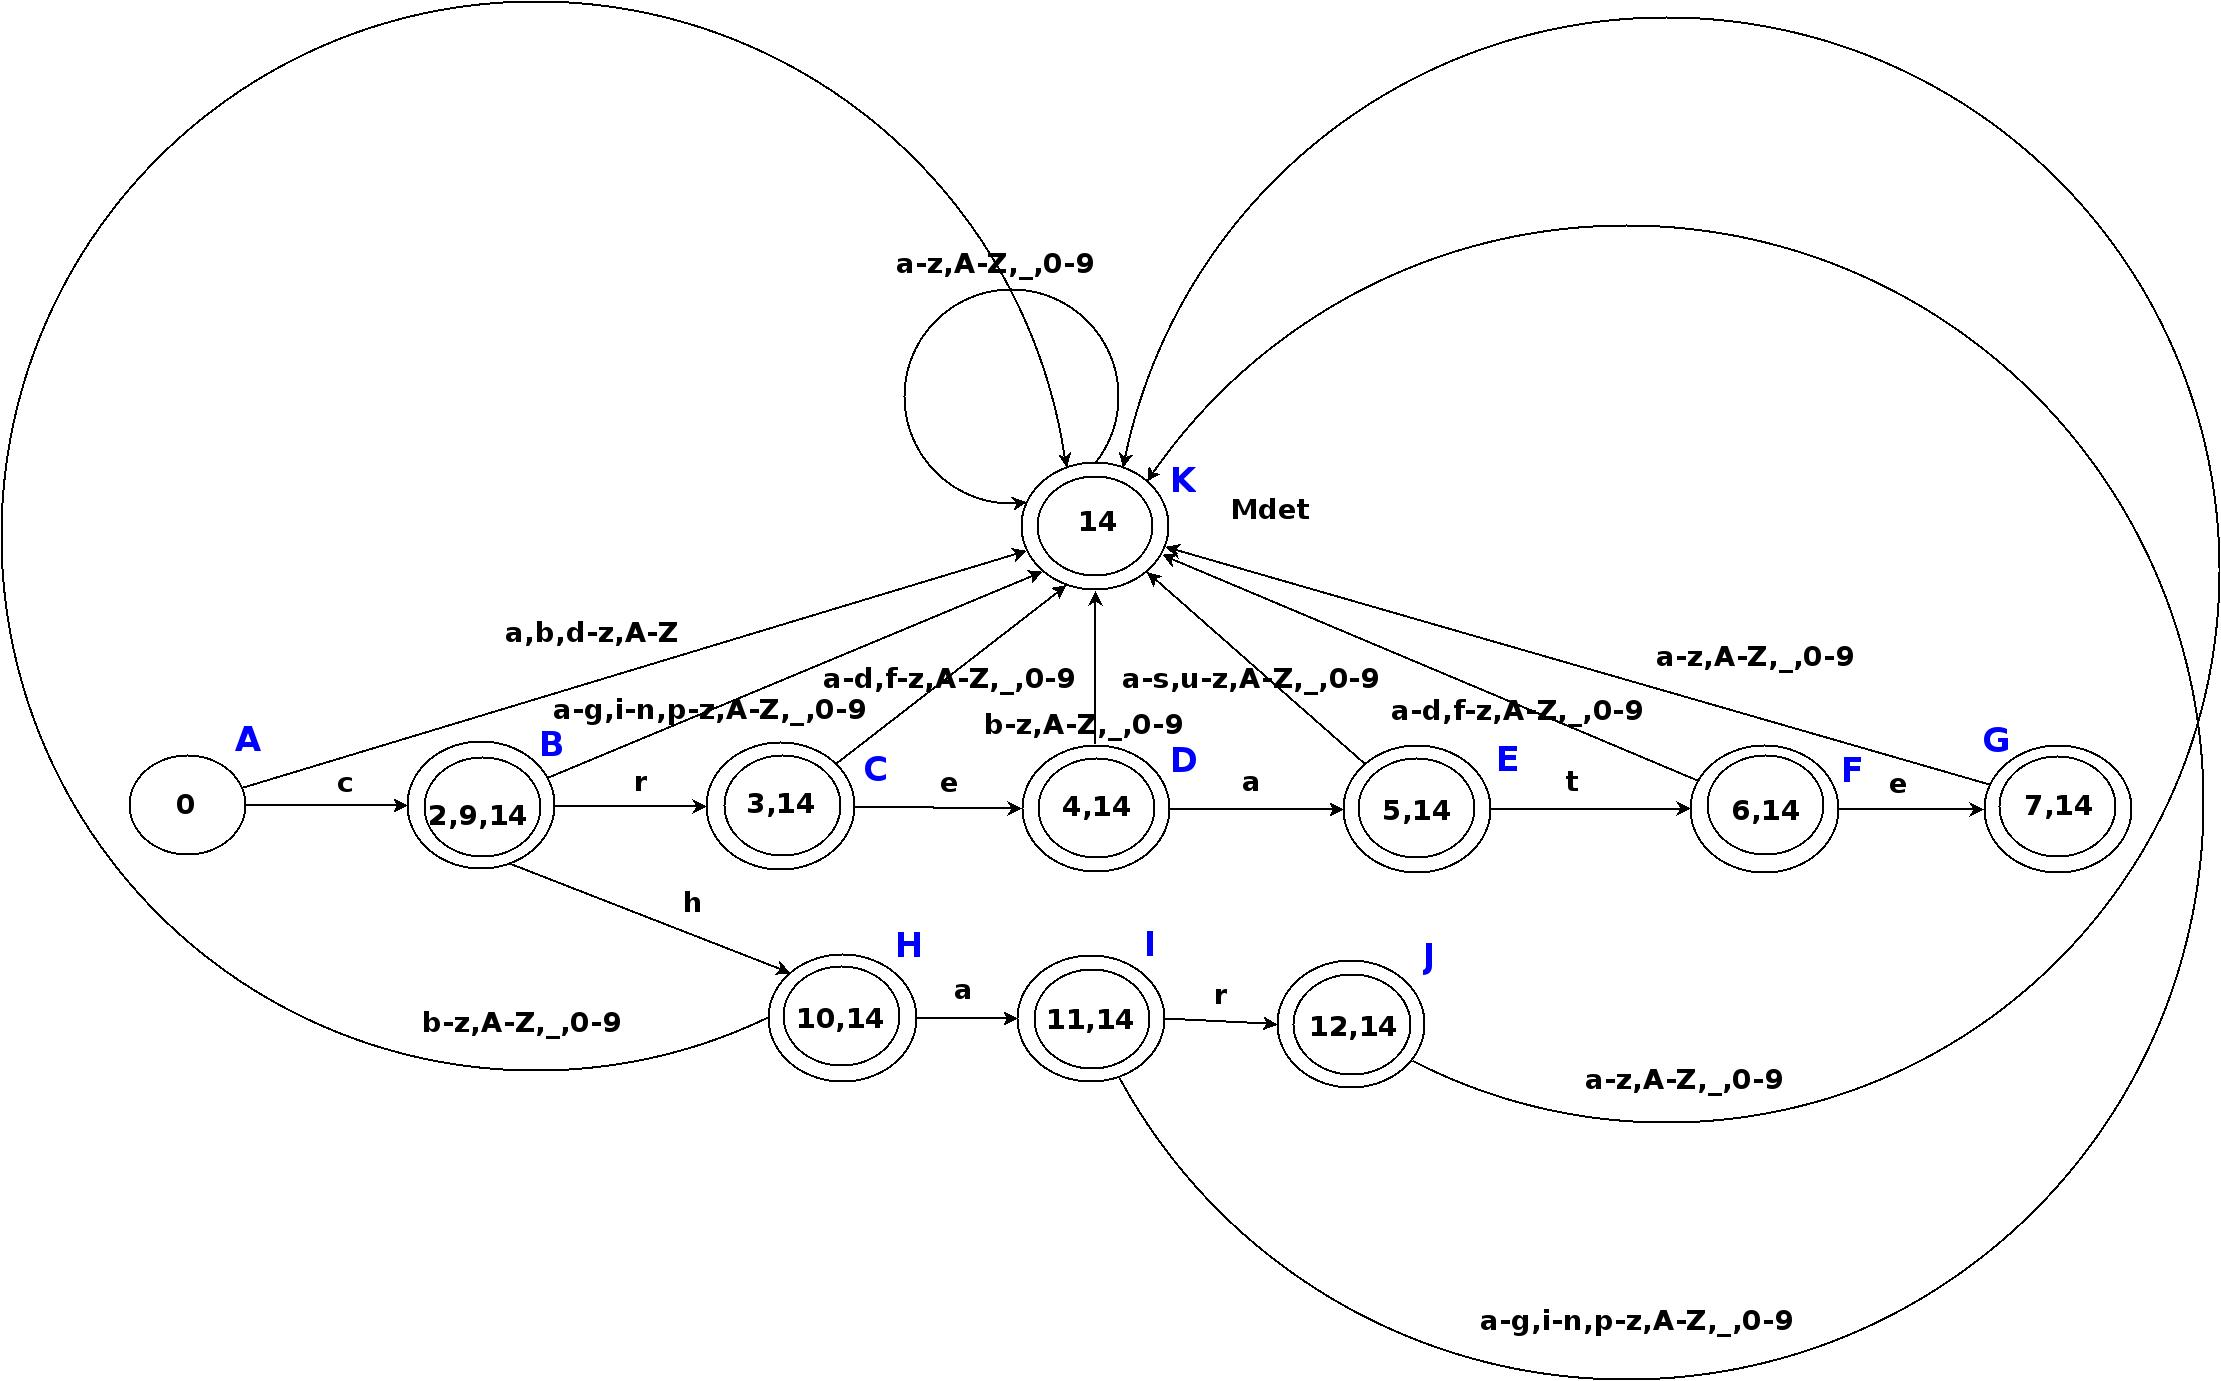
\includegraphics[scale=0.2]{preg6} 

\subsection{Pregunta 7}
\hspace{0.5cm} En el autómata Mdet, los conflictos ya no existirían, ya que sabemos que una vez que se llegue al estado final 7,14 corresponde a la palabra completa reservada create, al igual que para el estado final 12,14 que corresponde a la palabra reservada char. Por lo tanto el haber creado éste autómata determinístico nos muestra como se ha podido solucionar los conflictos anteriores existentes.

\subsection{Pregunta 8}
\hspace{0.5cm} Análogamente a la pregunta 4, para el lenguaje L(E1), le corresponde el estado final 7,14; para L(E2), le corresponde el estado final 12,14; y finalmente para L(E3), le corresponde el estado final 14.

\subsection{Pregunta 9}
\hspace{0.5cm} Para construir nuestro autómata determinístico mínimo Mmin, necesitamos las respectivas clases de equivalencias que son las siguientes: \\  \\ 
=0 = \{ \{A\}, \{B,C,D,E,F,H,I,K\}, \{J\}, \{G\} \} \\
=1 = \{ \{A\}, \{B,C,D,E,H,K\}, \{I\}, \{F\}, \{J\}, \{G\} \} \\ 
=2 = \{ \{A\}, \{B,C,D,K\}, \{E\}, \{H\}, \{I\}, \{F\}, \{J\}, \{G\} \} \\
=3 = \{ \{A\}, \{C,K\}, \{B\}, \{D\}, \{E\}, \{H\}, \{I\}, \{F\}, \{J\}, \{G\} \} \\ 
=4 = \{ \{A\}, \{C\}, \{K\}, \{B\}, \{D\}, \{E\}, \{H\}, \{I\}, \{F\}, \{J\}, \{G\} \} \\


Por ende, podemos observar que Mdet es el Mmin pedido. Y de forma análoga a la pregunta 8, para L(E1) corresponde el estado final 7,14, para L(E2) corresponde el estado 12,14 y para L(E3) corresponde el estado 14.
 
\subsection{Pregunta 10}
\hspace{0.5cm} La relación entre el analizador lexicográfico implementado con Ply y las preguntas respondidas anteriormente, se encuentra en el hecho de que, el funcionamiento interno del analizador lexicográfico de Ply podría utilizar el algoritmo usado en las preguntas 1-9 para crear un autómata finito determinista mínimo que sirva para realizar el \textit{match} entre la entrada pasada al analizador, y las expresiones regulares que representan a cada token.  \\ 

De esta manera, es posible que en lexer de Ply, realize este proceso de manera interna, siempre recordando que lo hecho en las preguntas 1-9, sólo fue aplicado sobre 3 expresiones regulares. En la realidad, el proceso es realizado sobre cada expresión regular que represente a cada token del lenguaje, lo cual probablemente genere un autómata mínimo mucho más grande al resultante en la pregunta 9.

\newpage

\begin{thebibliography}{9}
\bibitem{PlyDoc} 
David M. Beazley - Documentación de Python-PLY
http://www.dabeaz.com/ply/

\bibitem{Libro}
T. Sudkamp. Languages and Machines . Second Edition. Addison-Wesley, 1997.



\end{document}

